\documentclass{article}
\usepackage{color}
\usepackage{placeins}
\usepackage{listings}
\usepackage{graphicx}
\usepackage{xcolor}
\usepackage{amsmath}
\usepackage{subcaption}
\usepackage{cleveref}
\usepackage{geometry}[margins=1in]
\setlength{\parskip}{4pt plus 2pt}
\setlength{\parindent}{0pt}
%\pagecolor[rgb]{0,0,0} %black
%\color[rgb]{1,1,1} %grey
\lstset{language=C++,
keywordstyle=\color{blue},
stringstyle=\color{red},
commentstyle=\color{green},
morecomment=[l][\color{magenta}]{\#},
breaklines=true,
breakatwhitespace=true,
numbers=left
}
\title{Assignment \#2}
\author{Asbjørn Bonefeld Preuss,\\ Daniel Lomholt Christensen,\\ Elie Cueto}
\date{February 2024}
\setlength{\textheight}{1.05\textheight}
\begin{document}
\maketitle
\section{Task 1: Create a Struct-of-Arrays version of the program (amenable to
vectorisation)}
Before we can change the structure of the code to make it amenable to vectorisation by using SoA, we must first figure out where the code uses AoS, and where it does computations on these.

\subsection{The data structure}
In the \texttt{Water\_sequential.cpp} file, the classes \texttt{Atom}, \texttt{molecule}, and \texttt{System} are the biggest sinners. Each atom has its own mass, $\epsilon$, $\sigma$, charge, name, position vector, velocity vector, and force vector. Each molecule then has its own three atoms, two bonds and one angle. The system then consists of a vector of molecules, each consisting of a vector of atoms, each containing a number of properties and several vectors. We can change this up quite a bit: 

Each molecule is identical, so we can make three vectors of atoms, one for the O-atoms, one for the left H-atoms, and one for the right H-atoms. This is what we do in the \texttt{Molecules} class on lines $129$--$135$. This allows for calculating bond and angle forces in a vectorised manner, and will also help with the non-bond forces.

Each type of atom has identical values for mass, $\epsilon$, $\sigma$ and charge, and names so storing these as a parameter of this type instead of individual atoms optimises memory use. Furthermore, the position was changed from a \texttt{Vec3} to an array for each coordinate, thus keeping multiple positions in cache memory. This is done for the \texttt{Atoms} class on lines $110$--$126$. Now the \texttt{System} class on lines $141$--$145$ just contains a \texttt{Molecules} object and the simulation time.

\subsection{Computations}
Next up we want to alter the functions in our simulation to be able to take advantage of the new data structure. 

In the function \texttt{UpdateBondForces} on lines $186$--$203$, the original function takes one molecule at a time, and calculates the two bond forces before moving on to the next molecule. Now we are storing all the left H-to-O bonds together, and all the right H-to-O bonds together, so instead we let the outer loop be over the bonds, and the inner loop be over the molecules. Now we first calculate all the left bond forces, then all the right bond forces, which can be done in a vectorised manner now due to how bonds are stored.

In the function \texttt{UpdateAngleForces} on lines $207$--$251$, we do the exact same thing as above in \texttt{UpdateBondForces}. The outer loop is now over angles, the inner loop is over the molecules, and the convenient data structure now lets the function be vectorised.

The function \texttt{UpdateNonBondedForces} on lines $255$--$290$ is where the brunt of the changes take place. The function calculates the coulomb and Lennard Jones interactions between each pair of atoms, and therefore is has to do $O(N^2)$ computations,  where the above functions only had to do $O(N)$, so this is also the function we would expect to be the most time consuming when running the program.

%Originally, the function had its outermost loop over each molecule $M_i$, then each other molecule $M_j,j>i$, then each atom in $M_i$ and then each atom in $M_j$. This causes a lot of jumping around in the memory for the sequential program. What we do instead is to swap the two sets of loops, so we now have the outermost loops on lines $259$--$260$ over each atom in $M_i$ and $M_j$, and the innermost loops on lines $267$ and $272$ over each molecule pair $M_i$ and $M_j,j>i$. This means that we first take all the O-atoms, and find their interactions with all the other O-atoms, and then their interactions with all of the left H-atoms, and then with all the right H-atoms. Then we do the same for all the left H-atoms and then for all the right H-atoms.

We calculate interactions between like atoms, first, to make better use of the cache memory. Because the atoms are stored with all the O-atoms together and so on, this lets the code vectorise. One small drawback to this is that previously, when calculating the effect on one atom of all the atoms in another molecule, the effects generally added up to something very close to zero. Now, the combined effect when a lot of identical atoms from different molecules is found at once, the much larger numbers involved mean that small numerical errors can be introduced, which will cause the results to be slightly different when doing many calculations.

Next up, we see that in the original code $\epsilon_{ij}$ and $\sigma_{ij}$ was calculated for each pair of atoms, even though they are the same most of the time. Particularly as we are now finding the interactions of e.g. all the O-atoms wit all the other O-atoms at once, we only need to calculate $\epsilon_{ij}$ and $\sigma_{ij}$ once as we now do on lines $261$--$262$. As $\sigma_{ij}$ only appears squared, and as the charges only appear as $q_iq_j$, we can also just calculate these once, as we do on lines $263$--$264$.

Next, we have changed the way positions are stored, so each atom's position is not stored in its own vector, but the entire code is still very much built around using the \texttt{Vec3} type, so to avoid rewriting the whole program, we instead make a pair of vectors on lines $273$--$274$, which contain the positions of the two atoms in question. Finally, as the quantity $\frac{\sigma}{r}$ only appears to the 6'th or 12'th powers, we define \texttt{sir3} on line $280$ as $\left(\frac{\sigma}{r}\right)^6$, in order to minimise the number of needed operations.

The function \texttt{Evolve} on lines $293$--$316$ gets the same treatment as desctibed above. loops are swapped on lines $298$--$299$ so the outer loop is over atom types and the inner loop is over molecules, a position vector is created on lone $300$ to avoid having to rewrite large chunks of the code, and the updated position vector is put back in place on line $304$.

Finally the \texttt{MakeWater} function on lines $319$--$360$ has been altered to account for the new data structure. on lines $331$--$333$ we define the atoms in the new \texttt{atoms} class instead of the old \texttt{atom} one. On lines $349$--$351$ the initial positions are put in the separate x, y, and z vectors, instead of each atom having its own position vector. 

Finally on line $348$ the initial positions are now a spiral pattern rather than a line, to make the problem actually 3D. This has nothing to do with vectorisation, but we figured that not having a third of the number just be zero all the time might make a difference.

\section{Task 2: Investigate the performance of the code with a profiler}
Answer to the questions posed in the assignments:
\begin{itemize}\setlength{\itemsep}{0pt}
    \item The sequential simulation, run with 4 molecules for 100,000,000 time steps, spent 70.83\% of the time in UpdateNonBondedForces, whilst the vectorised simulation spent 74.25\% of the time in UpdateNonBondedForces. The profiler used was \texttt{gprof}, and the visualised profiling can be seen on figures \ref{fig: seq profile 2 molecule} through \ref{fig: seq profile 128 molecule}
    \item The sequential one spent less time in UpdateNonBondedForces when run with 2 molecules (43.99\%), whilst with 16 it spent more time in it at 92.69\% and even more when run with 128 molecules at 98.98\% of the time.
    
    The same thing happened with the vectorised simulation, where the simulation with 2 molecules yielded a spent percent time of 50.79\%
    in UpdateNonBondedForces, 16 molecules spent 92.97\%
    percent in UpdateNonBondedForces, and finally 128 molecules spent 98.71\% 
    in UpdateNonBondedForces. The profile images can be seen in the appendix, from figure \ref{fig: vec profile 2 molecule} through \ref{fig: vec profile 128 molecule}.

    All in all, UpdateNonBondedForces is the most demanding function, and this is because it scales quadratically, rather than linearly as UpdateAngleForces and UpdateBondForces do.

    \item There is a difference between the vectorised and sequential functions, as the vectorised optimizes the UpdateNonBondedForces quite heavily. Accessing all the atoms of the same type, after each other, allows for the atoms to be read in the same cache, thus increasing the load in time of the function.
\end{itemize}


\section{Task 3: Adding OpenMP SIMD pragmas to the code}
By compiling the code with the flag \texttt{-fopt-info-vec-optimized}, we get info about where the compiler is vectorising loops. We find that the \texttt{Atoms} class on line 110 is vectorised, although this will hardly make a huge difference. 

We also see that a loop on line 193 is versioned for vectorisation in the $\texttt{UpdateBondedForces}$ function, but the compiler is careful here, as there is a running sum in the loop. Therefore we add here the pragma \texttt{\#pragma omp simd reduction(+:accumulated\_forces\_bond)}. Adding this pragma makes the code vectorise the loop with no issues.

Next we come to the part of the code that takes up around $99\%$ of the computation time, the \texttt{UpdateNonBondedForces} function on lines $255$--$290$. This does not get vectorised on its own. This is due to the loop containing several running sums, one if which is a \texttt{Vec3} sum of an element of a vector inside a class. The compiler has a number of issues with this, but we can tell the compiler how to do a reduction on a \texttt{Vec3} type by using the pragma \texttt{\#pragma omp declare reduction(+:Vec3:omp\_out += omp\_in) initializer(omp\_priv = omp\_orig)} on line $270$. Then we create a new variable \texttt{Vec3 af} on line $269$ to hold the sum, instead of having the reduction directly on an array element. Now we add the pragma \texttt{\#pragma omp simd reduction(+:accumulated\_forces\_non\_bond,af)} on line $271$, which allows the loop to be vectorised properly. 

The main loop in the program - i.e. the loop that takes up the vast majority of the computation time - is now vectorised, but the runtime improvements are minor due to the original program already being very well written.
\newpage
\appendix
\section*{Figures for profiling the code}
\FloatBarrier
\begin{figure}
    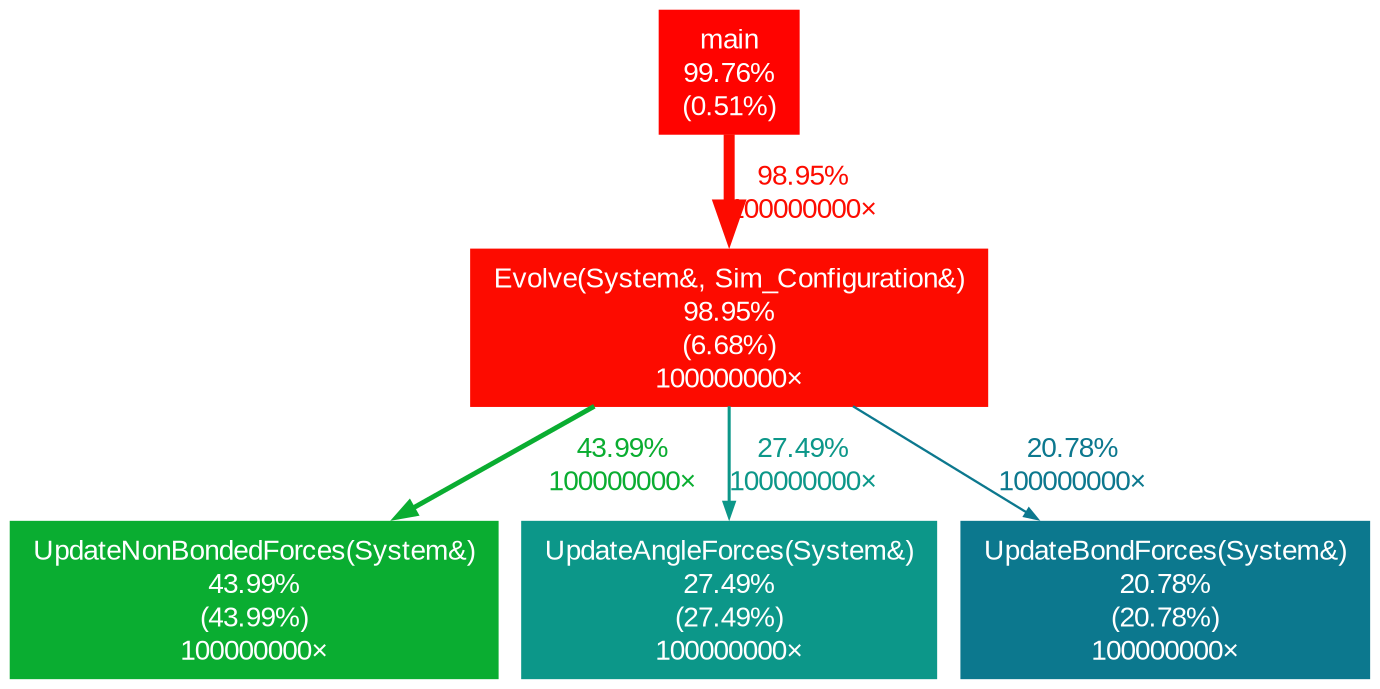
\includegraphics[width=0.7\textwidth]{Images/seq_2mol_profile.png
    }
    \centering
    \caption{Profile image of the sequential simulation run with 2 molecules}
    \label{fig: seq profile 2 molecule}
\end{figure}

\begin{figure}
    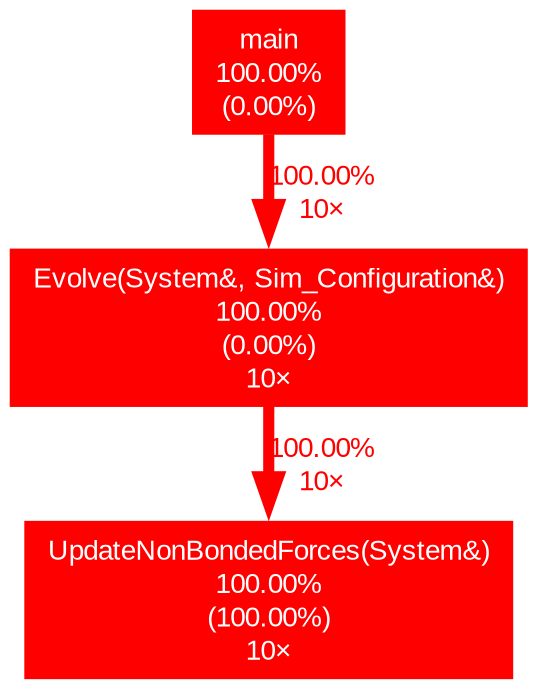
\includegraphics[width=0.7\textwidth]{Images/vec_4mol_profile.png}
    \centering
    \caption{Profile image of the sequential simulation run with 4 molecules}
    \label{fig: seq profile 4 molecule}
\end{figure}
\begin{figure}
    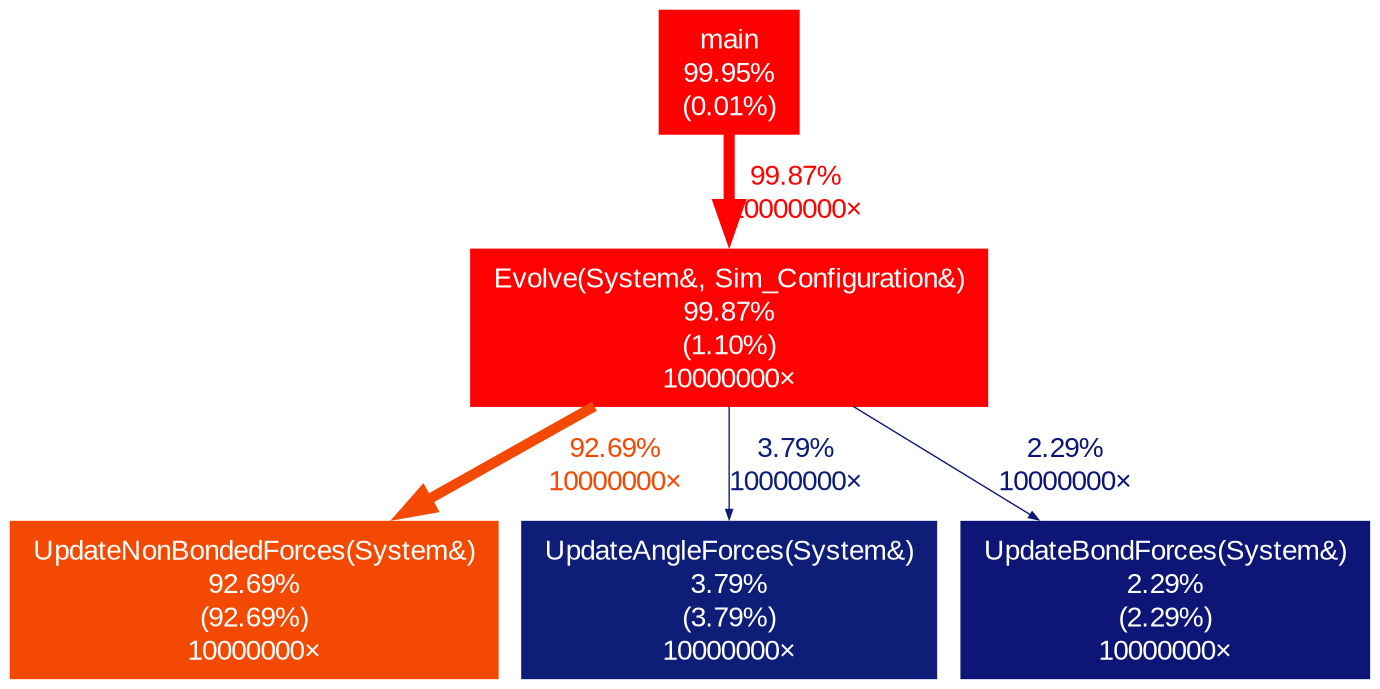
\includegraphics[width=0.7\textwidth]{Images/seq_16mol_profile.png
    }
    \centering
    \caption{Profile image of the sequential simulation run with 16 molecules}
    \label{fig: seq profile 16 molecule}
\end{figure}
\begin{figure}
    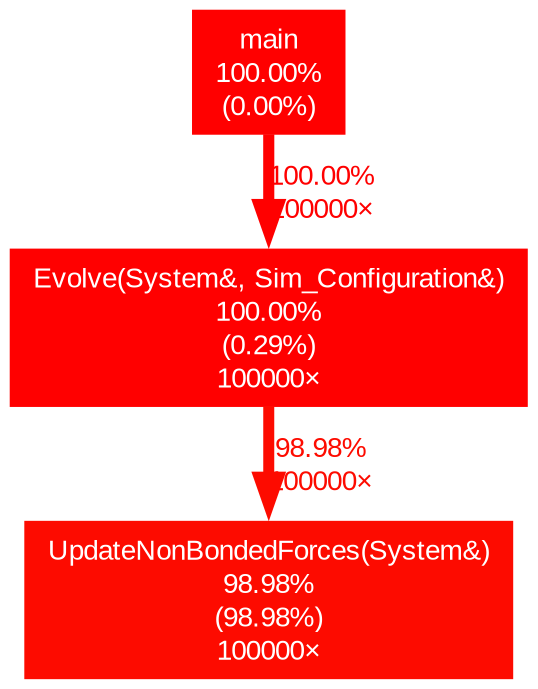
\includegraphics[height=0.5\textheight,width=0.7\textwidth]{Images/seq_128mol_profile.png
    }
    \centering
    \caption{Profile image of the sequential simulation run with 128 molecules}
    \label{fig: seq profile 128 molecule}
\end{figure}

\begin{figure}
    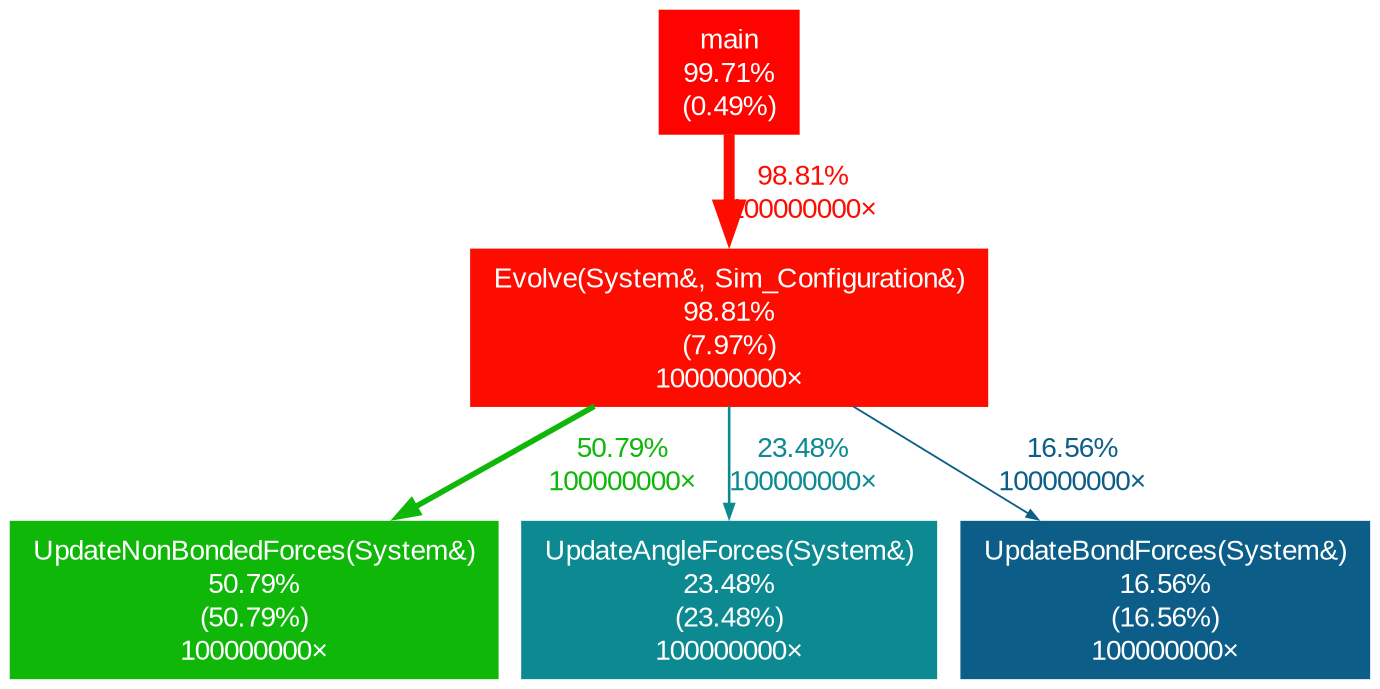
\includegraphics[width=0.7\textwidth]{Images/vec_2mol_profile.png
    }
    \centering
    \caption{Profile image of the vectorised simulation run with 2 molecules}
    \label{fig: vec profile 2 molecule}
\end{figure}

\begin{figure}
    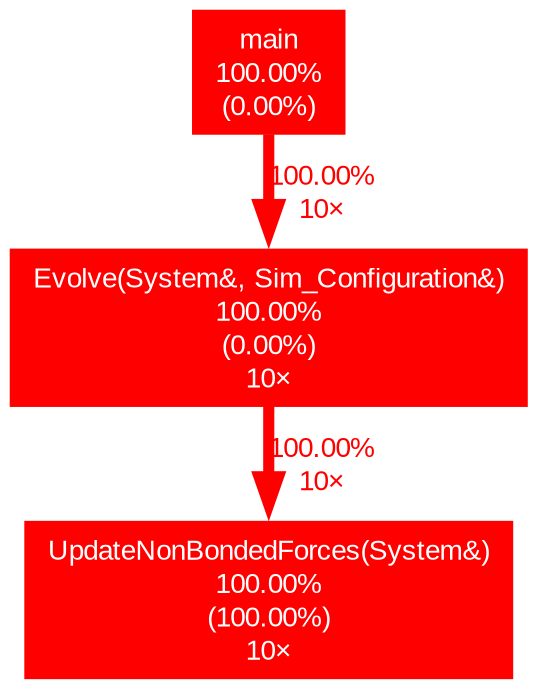
\includegraphics[width=0.7\textwidth]{Images/vec_4mol_profile.png}
    \centering
    \caption{Profile image of the vectorised simulation run with 4 molecules}
    \label{fig: vec profile 4 molecule}
\end{figure}
\begin{figure}
    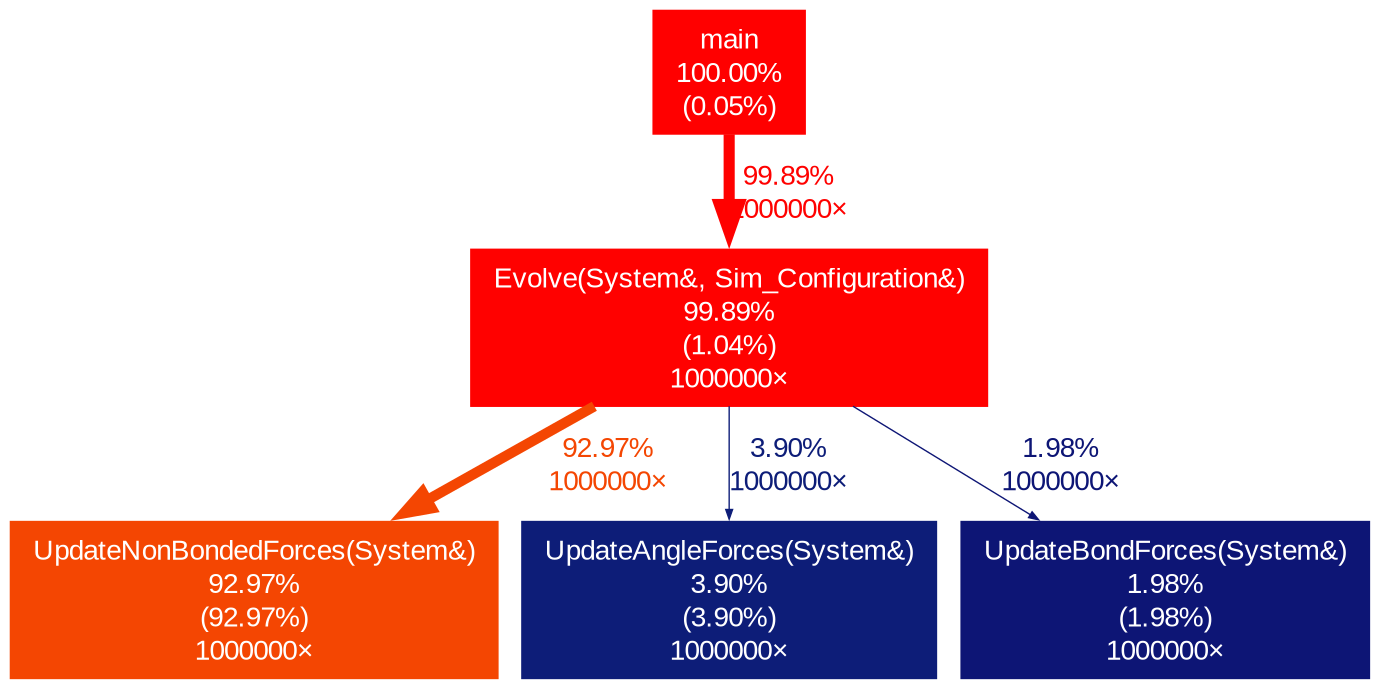
\includegraphics[width=0.7\textwidth]{Images/vec_16mol_profile.png
    }
    \centering
    \caption{Profile image of the vectorised simulation run with 16 molecules}
    \label{fig: vec profile 16 molecule}
\end{figure}
\begin{figure}
    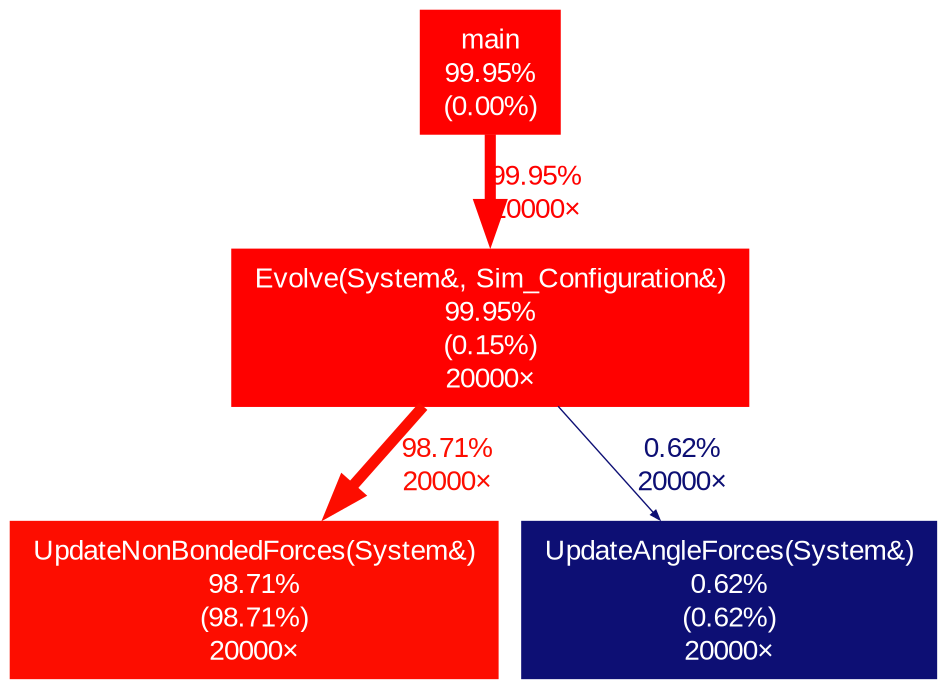
\includegraphics[width=0.7\textwidth]{Images/vec_128mol_profile.png
    }
    \centering
    \caption{Profile image of the vectorised simulation run with 128 molecules}
    \label{fig: vec profile 128 molecule}
\end{figure}


\FloatBarrier
\section*{Source Code}
\lstinputlisting[language=c++]{../Code/Water_vectorised.cpp}

\end{document}
